\documentclass{article}

\usepackage{geometry}
\geometry{letterpaper, total={7in, 10in} }
\usepackage{booktabs}
\usepackage{graphicx}
\usepackage{verbatim}

\title{CSCI 4360 Data Science II Project I}
\author{Ayush Kumar, Faisal Hoissain, Brandon Amirouche}
\date{February 23, 2021}

\begin{document} 
	
	\maketitle
	\tableofcontents
	
	\section{Introduction and Methodology}
	\subsection{Code Credits}
	\section{Auto-MPG}
	\section{Concrete Compressive Strength} 
	\section{Crime}
	\section{Wine Quality}
	\subsection{The Dataset} 
	
	The wine quality data is actually two datasets, one for red wine and the other for white 
	wine. Both of them have the same 11 features, but there may be differences in the features 
	that matter, as well as the overall results of regression. A dummy variable could be created 
	to meld the datasets into one overall set, but if there are substantial differences between 
	the two it may substantially add to model complexity. The dataset has the following variables: 
	
	\begin{enumerate}
		\item fixed.acidity 
		\item volatile.acidity 
		\item citric.acid 
		\item residual.sugar 
		\item chlorides 
		\item free.sulfur.dioxide 
		\item total.sulfur.dioxide 
		\item density
		\item pH
		\item sulfates 
		\item alcohol 
		\item quality (the response variable)
	\end{enumerate}

	The red wine dataset has 1,599 observations, and the white wine dataset has 4,898 observations. 
	The two files can be found in the data/WineQuality folder, and were orignally downloaded from 
	the UCI Machine Learning Repository. [insert link here]

	\subsection{Exploratory Data Analysis}
	
	The first step in EDA was to checkout the collinearity of features, and how well they correlate 
	with our response variables. 
	
	
	\textbf{ Red Wine Correlation Matrix (Plotted with R)}
	
	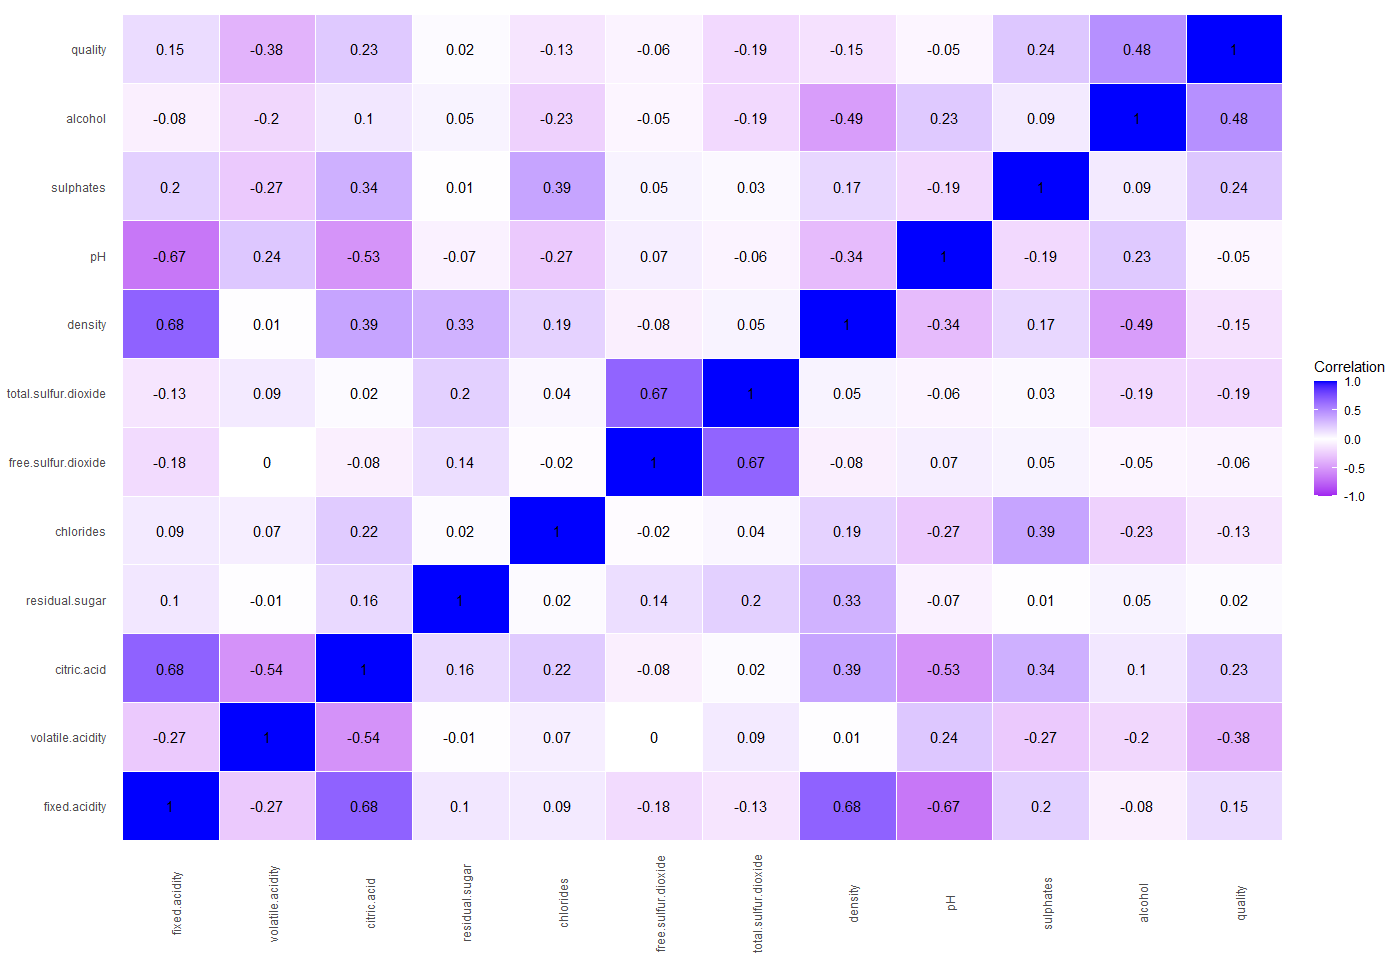
\includegraphics[scale=0.5]{../plots/Wine/red_wine_Rcormat.png}

	From the Red Wine Correlation Matrix (Figure 1) we can see that there are a few variables that have fairly strong 
	correlations with each other. The citric acid content and the fixed acidity seem to be highly correlated 
	with each other, and this pattern holds true for many of the features that depend on acidity. We can see 
	that pH is highly correlated with fixed acidity and citric acid as well. This will be important to consider 
	as it may create a problem in our regression. Based on the results of our variable screening methods, we may
	consider dropping one or more these variables, or using them as an instrumental variable to reduce the 
	endogeneity issue with this dataset. Another highly correlated issue may be density and fixed acidity, as well 
	as free.sulfur.dioxide and total sulfur dioxide. It may be worth our time to standardize some of these 
	variables to limit collinearity, and this will be considered during variable selection. 
	
	\newpage
	\textbf{ White Wine Correlation Matrix (Plotted with R)}
	
	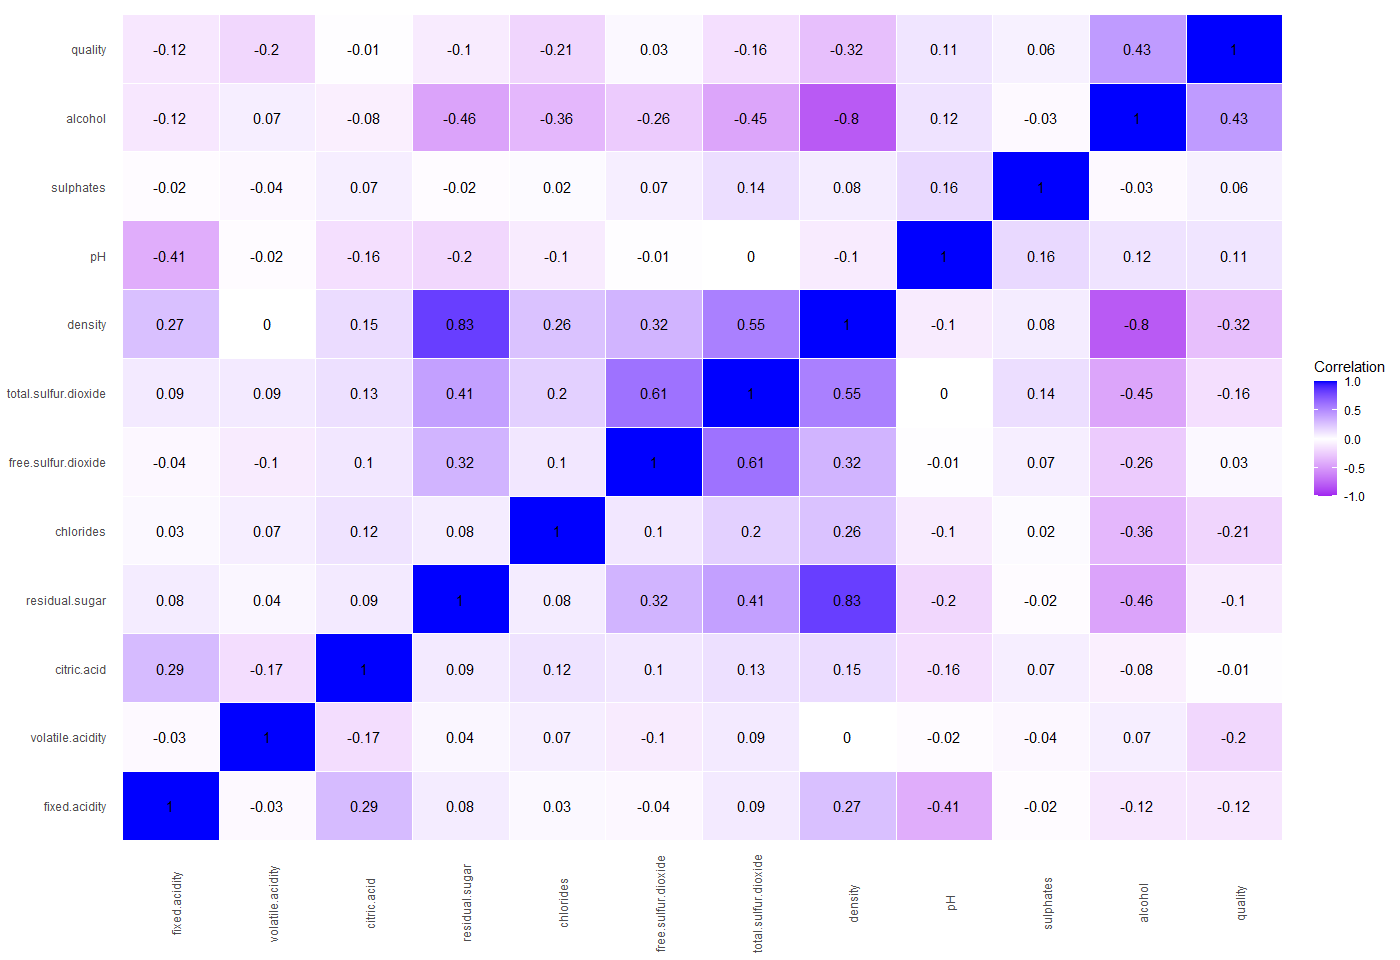
\includegraphics[scale=0.5]{../plots/Wine/white_wine_Rcormat.png}

	
	Moving on to the white wine dataset, we can see very clearly that the behavior is very different from the collinearity 
	between variables is quite high for two interactions in specific. The first is between density and residual sugar, the 
	second is between alcohol and density. Both of these are higher than 0.8, but residual sugar seems to have very little 
	correlation with our response variables, so it may not end up being an issue after variable selection. The high 
	correlation between alcohol and density seems to pose a much more substantial issue because both have some 
	correlation with quality of the wine. We may standardize one or both of these variables during variable 
	screening, or remove one of them from our regression on the basis of our 4 criterion. 
	
	\newpage 
	
	\textbf{Red Wine Scatter Plots (R)}
	
	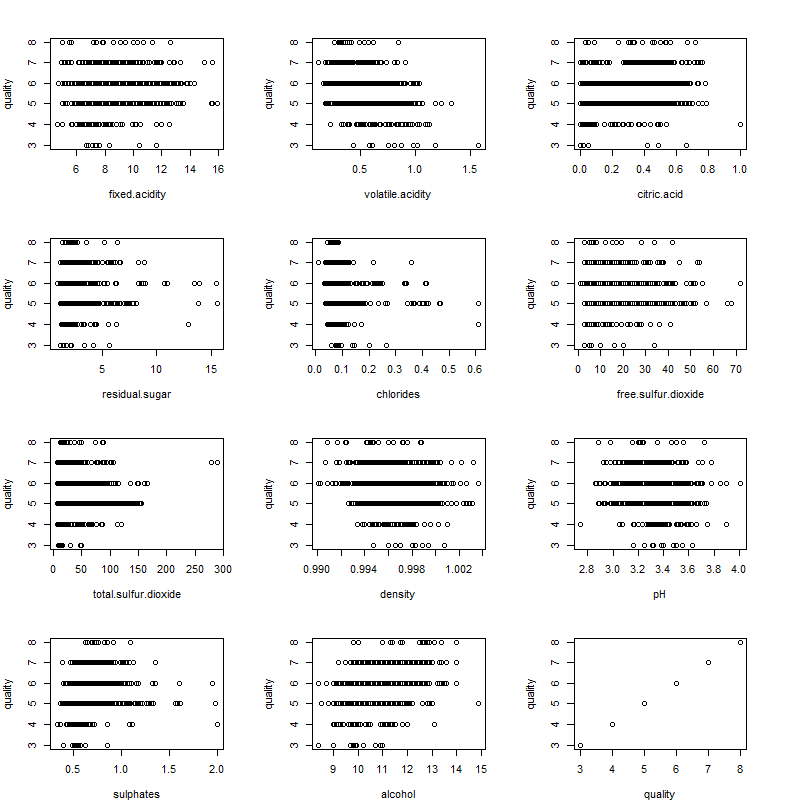
\includegraphics[scale=0.7]{../plots/Wine/red_wine_Rscatter.png}
	\newline
	
	Quality seems to be a multi-categorical variable, based on this information maybe regression is not the best
	way to predict on this dataset, but it may give a great deal of information regarding feature selection. Some
	features exhibit very peculiar behavior of having similar characteristics for both low and high quality wines, but
	not for middle quality wines. This can be illustrated when we take a look at total sulfur dioxide, chlorides, and 
	residual sugar. This pattern may mislead us during variable selection, so it may be a good idea to add in 
	quadratic terms for these variables to account for their curving behavior. If these variables fail to be selected 
	initially then I will rerun variable selection methods taking into account their quadratic terms. There may 
	be other transformations needed, but we can determine those after variable selection bases on partial residual 
	plots. 
	
	\newpage
	
	\textbf{White Wine Scatter Plots (R)} 
	
	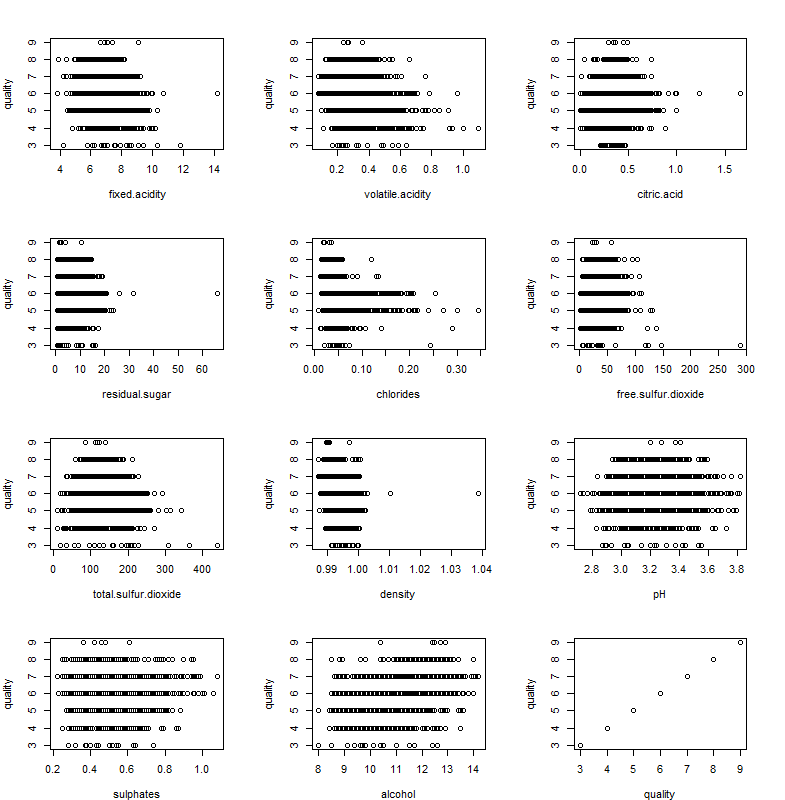
\includegraphics[scale=0.7]{../plots/Wine/white_wine_Rscatter.png}
	
	We once again see very similar patterns to the first dataset in terms of residual sugar, chlorides, and
	sulfur dioxide. There does not seem to be anything else out of the ordinary in these scatterplots. Taking 
	this into account the obvious next step is variable screening and selection. 

	\subsection{Variable Screening and Selection}
	

	\textbf{Variable Selection for Red Wine} 
	
	
		Output has been modified for space. Run code for full output. 
	\verbatiminput{../R/output/wine/red_forward_selectionR.txt}

	One of the variables that was omitted here was residual sugar, one of the variables that exhibited very strong 
	quadratic behavior. I will be rerunning forward selection while including the quadratic term for residual sugar 
	and it will be included for all of the following variable selection methods as well. This is the final call when 
	I include the quadratic term in the forward step. 
	
	\begin{verbatim}
			Call:
				lm(formula = quality ~ alcohol + volatile.acidity + sulphates + 
				total.sulfur.dioxide + chlorides + pH + free.sulfur.dioxide, 
				data = red_wine)
	\end{verbatim}
	
	As can be seen even the inclusion of the quadratic term did not change the results of the forward selection. Below
	are listed the final conclusions of backwards elimination and step wise regression. 
	
	\textbf{Backward Elimination}
	\begin{verbatim}
			Call:
				lm(formula = quality ~ volatile.acidity + chlorides + free.sulfur.dioxide + 
				total.sulfur.dioxide + pH + sulphates + alcohol, data = red_wine)
	\end{verbatim}
	
	\textbf{Step Regression} 
	\begin{verbatim}
			Call:
				lm(formula = quality ~ alcohol + volatile.acidity + sulphates + 
				total.sulfur.dioxide + chlorides + pH + free.sulfur.dioxide, 
				data = red_wine)
	\end{verbatim}
	
	
	While the methods may be different every single one of our variable screening methods chose the same seven variables 
	to include: alcohol, volatile.acidity, sulphates, total.sulfur.dioxide, chlorides, pH, and free.sulfur.dioxide. These 
	are the variables that will be included in all our models for red wine moving forward. 
	
	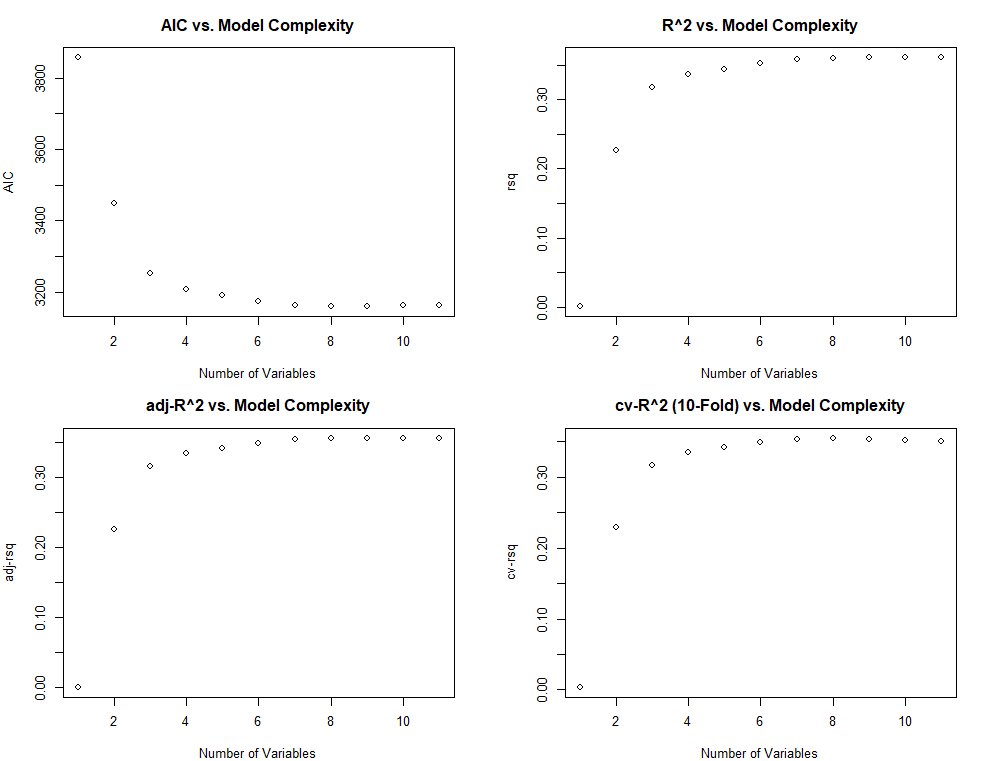
\includegraphics[scale=.55]{../plots/Wine/qof_plotR.png}
	
	Here we can see that as we increase the number of variables, we see diminishing marginal improvement in quality of 
	fit. For measures that penalize model complexity such as $R^2$ and AIC we can even see a light bend towards 
	the quality of fit worsening as model complexity increases. The diminishing returns can in part be explained by 
	variables that have weak correlation 
	
	
	\textbf{Variable Selection for White Wine}
	
	\section{Seoul Bike Rentals}
	\section{Air Quality}
	
	
\end{document}